\documentclass[orivec,runningheads]{llncs}
\usepackage[T1]{fontenc}
\usepackage{graphicx}
\usepackage{booktabs}
\usepackage[misc]{ifsym}
\usepackage{xcolor}
\newcommand{\corr}{(\Letter)}
% N.B.: do not change anything above this line. If you require additional packages, please load them directly after this line.

\usepackage{amsmath}
\usepackage[utf8]{inputenc} % allow utf-8 input
\usepackage[colorlinks=true, allcolors=blue]{hyperref}       % hyperlinks
\usepackage{url}            % simple URL typesetting
\usepackage{amsfonts}       % blackboard math symbols
\usepackage{nicefrac}       % compact symbols for 1/2, etc.
\usepackage{microtype}      % microtypography
\usepackage{xcolor}         % colors
\usepackage{graphicx}
\usepackage{float}
\usepackage{bm}
\usepackage{bbm}
\usepackage{enumitem}
\usepackage[colorinlistoftodos]{todonotes}
\usepackage{mwe}
% N.B.: you may delete the preceding line. It is used to display an example image in this template.

% --- REQUIRED PACKAGES FOR TABLE FORMATTING ---
\usepackage{longtable}
\usepackage{booktabs}
\usepackage{array}
\usepackage{hyperref}

\DeclareMathOperator*{\dist}{dist}

\begin{document}

\title{A Simulation Framework for the Multi-Period Vehicle Routing Problem with Profits in Smart Waste Collection}

\titlerunning{A Simulation Framework for MPVRP w/ profits}
\authorrunning{A.C. Fernandes et al.}
% First names are abbreviated in the running head.
% If there is one author, write 'A.L. Benjamin'.
% If there are two authors, write 'A.L. Benjamin and C.C. Broadus Jr.'
% If there are more than two authors, '[...] et al.' is used.

\institute{INESC-ID, Lisboa, Portugal \email{afonso.fernandes@inesc-id.pt}
\and
Instituto Superior T\'ecnico, Universidade de Lisboa, Lisboa, Portugal \email{afonso.fernandes@tecnico.ulisboa.pt}
}
%\email{\{a.l.benjamin,a.a.patton\}@fsu.fake}}

\maketitle              % typeset the header of the contribution

\begin{abstract}
Urban waste collection is a critical municipal service with profound implications for sanitation and public health. This service heavily relies on vehicle routing and has traditionally been modeled as a static Capacitated Vehicle Routing Problem (CVRP), where vehicles perform an exhaustive collection of all bins. The introduction of smart waste bin monitoring technology has enabled dynamic vehicle routing, allowing vehicles to selectively visit only the subset of bins that require immediate service or are profitable to collect, a task which can be modeled as a Vehicle Routing Problem with Profits (VRPP). Furthermore, this task must be performed across an extended planning horizon, where routes executed in a given period impact the optimal routes for subsequent periods, forming a Multi-Period VRPP (MPVRPP). Because of the large scale and temporal dependencies, transferring existing CVRP solvers to this selective routing problem presents significant structural difficulties. Moreover, progress is currently hindered by a lack of standardized multi-period evaluation environments. To address these limitations, this paper introduces WSmartRoute+, a Python simulation framework designed specifically for the stochastic MPVRPP. Using this environment, a unified methodology is developed to adapt state-of-the-art CVRP algorithms - including Hybrid Genetic Search (HGS), Adaptive Large Neighborhood Search (ALNS), and recent Neural Combinatorial Optimization (NCO) models - to dynamic waste collection. The adaptations introduce novel profit-aware repair operators, and dynamic dispatch heuristics. To evaluate the generality of the proposed adaptations, an extensive benchmark of these classical and learning-based solvers is conducted. The experimental results establish a unified baseline for the MPVRPP and demonstrate WSmartRoute+ as a testbed for future research in dynamic, multi-period waste collection routing.
\end{abstract}

\section{Introduction}

Urban waste collection is a core public service with significant economic, environmental, and social implications. The operational planning of waste collection routes directly affects fuel consumption, labor costs, greenhouse gas emissions, service reliability, and citizen satisfaction. From a methodological standpoint, waste collection routing represents a particularly challenging class of vehicle routing problems, characterized by spatially distributed service points, capacity constraints, heterogeneous waste generation rates, and strict operational requirements.

Over the past decades, Operations Research (OR) has produced a wide range of optimization-based models and solution methods for waste collection routing, including exact formulations, decomposition approaches, and advanced heuristics \cite{hess2024waste,jorge2022hybrid,lopes2023efficient,de2024data}. While these approaches are capable of modeling realistic constraints and multiple objectives, their evaluation is typically conducted either on limited real instances or on static snapshots of the system. As a result, important operational aspects—such as daily variability in waste accumulation, interdependence between routing decisions over time, and the long-term effects of routing policies—are often neglected.

In parallel, recent advances in Deep Learning (DL) have given rise to Neural Combinatorial Optimization (NCO) methods, which aim to learn routing policies directly from data using deep neural networks trained via reinforcement learning \cite{wu2024neural}. These approaches have shown promising results on classical routing benchmarks, particularly when evaluated on synthetic and static problem instances. However, their applicability to real-world waste collection operations remains largely unexplored, due in part to the lack of realistic, dynamic, and reproducible evaluation environments.

A critical limitation of the current literature is the absence of simulation frameworks that faithfully capture the operational dynamics of waste collection systems. Real-world operations involve continuous waste accumulation, sensor uncertainty, service-level requirements, and feedback effects whereby routing decisions made on one day influence the state of the system on subsequent days. Without a simulation layer that explicitly models these dynamics, it is difficult to assess the true performance, robustness, and scalability of both OR-based solvers and learning-based routing policies.

To address this gap, this paper introduces a Waste Collection Routing Simulator designed to serve as a unified experimental platform for the development, evaluation, and comparison of routing strategies. The simulator integrates a dynamic system state that evolves over time, daily route execution, container-level waste accumulation processes, and multi-objective performance metrics reflecting real operational trade-offs. By decoupling the simulation of the operational environment from the optimization or learning components, the framework enables a fair and reproducible comparison between expert-crafted OR solvers and data-driven NCO models under identical conditions.

Within this simulator, routing decisions are not evaluated in isolation but as part of a sequential decision-making process, where each day's routes influence future system states, service feasibility, and performance outcomes. This perspective shifts the focus from solving single-shot routing problems to evaluating routing policies over extended planning horizons, which is more aligned with real-world waste management practice.

The proposed simulator is validated using real-world data from a waste management company operating across multiple municipalities in Portugal, involving instances with several hundreds of containers. It provides a realistic testbed for studying the strengths and limitations of both optimization-based and learning-based routing approaches, and supports systematic experimentation on scalability, robustness to uncertainty, and multi-objective trade-offs in waste collection operations.

This paper makes the following contributions:

\begin{itemize}
    \item We introduce a dynamic, multi-objective waste collection routing problem in which routing decisions influence the evolution of future problem instances through container-level waste accumulation and service constraints. This formulation naturally captures the sequential nature of real-world waste collection operations.
    
    \item We propose a modular Waste Collection Routing Simulator that enables the evaluation of routing policies under both blind and smart collection settings. The simulator supports stochastic waste generation processes, sensor uncertainty, and long-term policy evaluation over extended planning horizons.
    
    \item We develop and adapt Neural Combinatorial Optimization architectures for dynamic waste collection, including a lightweight attention-based model inspired by recommendation systems, and benchmark them against state-of-the-art expert-crafted OR solvers \cite{jorge2022hybrid,lopes2023efficient,de2024data}.
    
    \item We conduct an extensive computational study using real-world data from a Portuguese waste management company, considering networks of 100, 170, and up to 350 containers. The experiments analyze scalability, robustness to uncertainty, and trade-offs between operational cost, service level, and environmental impact.
    
    \item We systematically investigate the impact of different waste generation models, including Gamma distributions with varying parameters and empirical distributions derived from historical data, providing insights into how demand uncertainty affects the relative performance of static and dynamic routing policies.
\end{itemize}

\section{Problem Definition}
We model the Multi-Period Vehicle Routing Problem with Profits (MPVRPP) as a profit maximizing, multi-period constrained combinatorial optimization problem over a horizon of $D$ days. 

\subsection{Problem State and Dynamics}
Let $\mathcal{G} = (\mathcal{V}, \mathcal{E})$ be a fully connected graph where $\mathcal{V} = \{v_0, v_1, \dots, v_V \}$, with $v_0$ representing the depot and $\mathcal{V} \setminus \{v_0\}$ denoting the set of waste bins located at spatial coordinates $\vec{l}_i \in \mathbb{R}^2$. The state of the environment at day $d \in \{1, \dots, D\}$ is defined by the fill levels of the bins, denoted by the vector $\vec{w}_d = [w_{1, d}, \dots, w_{V, d}]^\top \in [0, \tau]^V$, where $\tau$ is the maximum bin capacity.

The waste $w_{i,d}$ accumulates stochastically according to a daily waste fill value sampled from a bin-specific distribution $\delta_{i,d} \sim P_i$. If a bin $v_i$ is visited on day $d$, its waste is collected and the level is reset; otherwise, waste continues to accumulate up to the bins' maximum capacity $\tau$:
\begin{equation}
    w_{i, d+1} = 
    \begin{cases} 
        \delta_{i, d+1} & \text{if } v_i \in \mathcal{A}_d \\
        \min(w_{i, d} + \delta_{i, d+1}, \tau) & \text{if } v_i \notin \mathcal{A}_d
    \end{cases}
\end{equation}

\begin{figure}
    \centering
    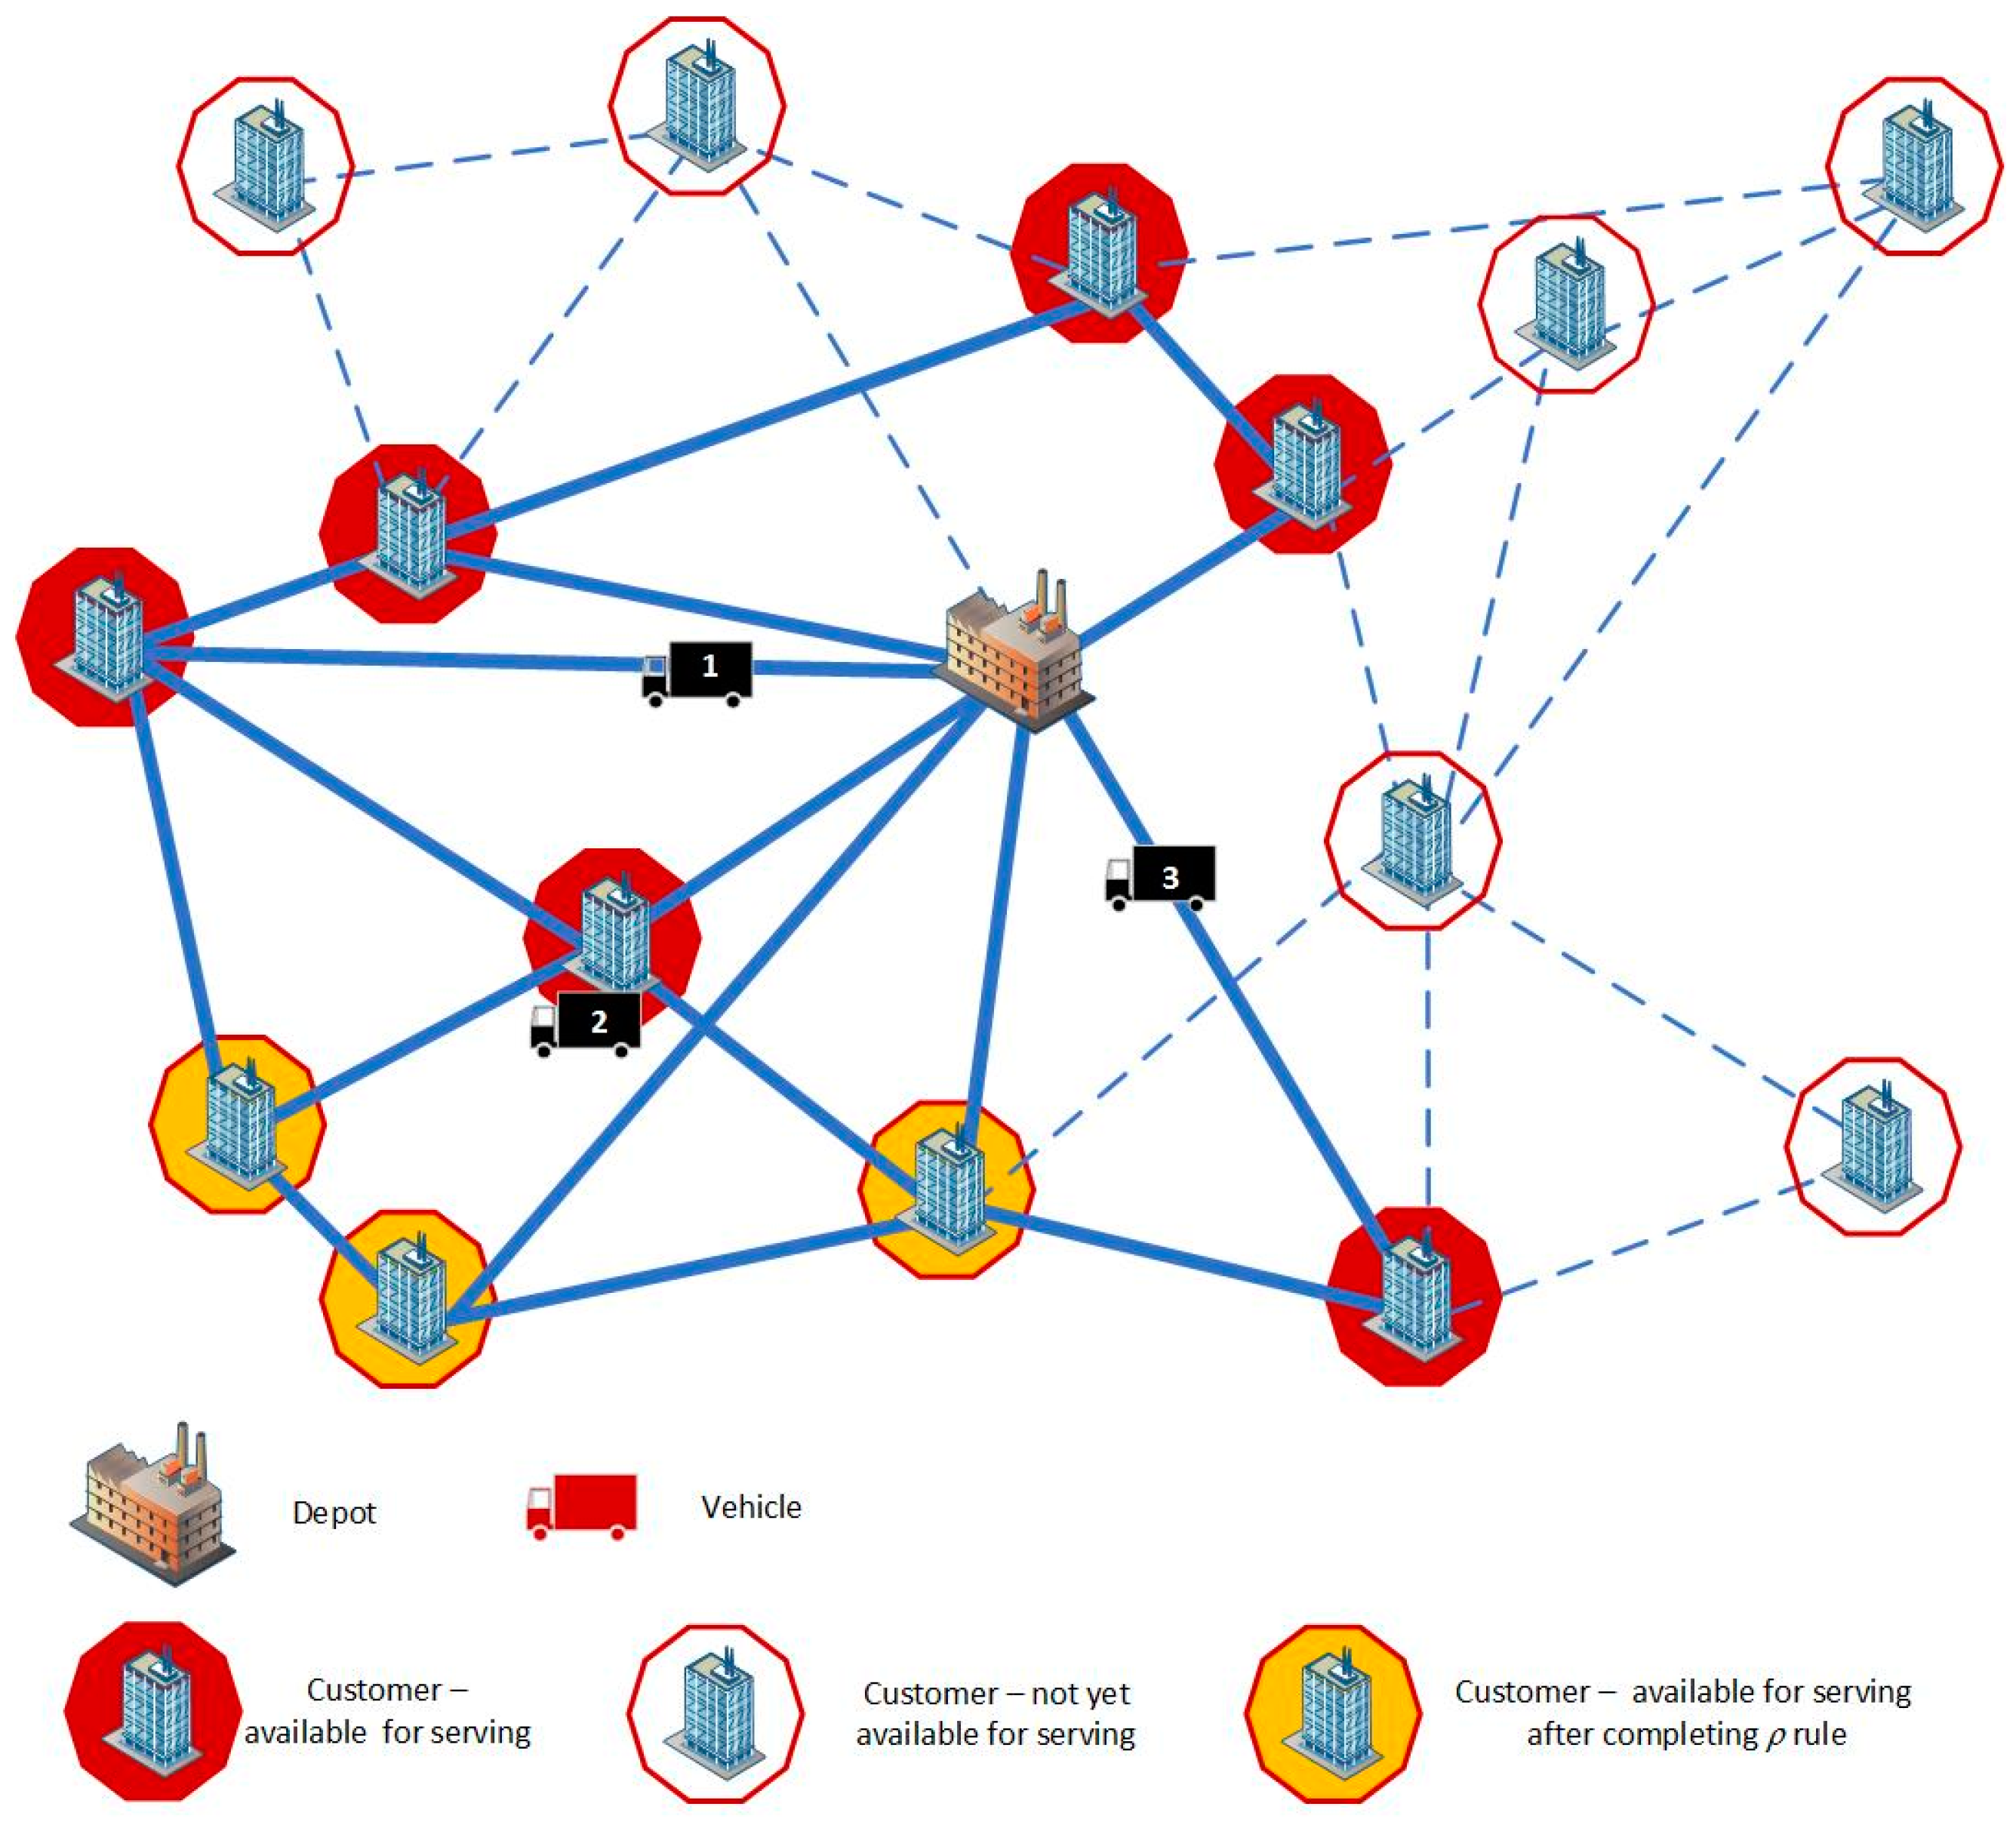
\includegraphics[width=0.75\linewidth]{Images/vrpp_multi_vehicle_example.png}
    \caption{Example of a single-day VRPP where multiple vehicles each serve a different subset of the selected bins. Figure adapted from \cite{sym11040546}.}
    \label{fig:vrpp_example}
\end{figure}

\subsection{Optimization Objective}

At each day $d$, the agent selects a (possibly empty) set $\mathcal{A}_{d}$ of bins to be visited distributed by $K$ routes, with each route starting and ending at the depot $v_0$:
\begin{equation}
    \mathcal{A}_{d,k} = (a_{0, k}, a_{1, k}, a_{2, k}, \dots, v_0).
\end{equation}

Here $a_{t,k}$ represents the action of visiting a certain bin on route $k$, with $a_{0, k} \equiv v_0$. The maximum number of routes can be limited by the resources available (vehicles). The constrained optimization problem for a single day can be formulated as finding the route(s) that:

\begin{equation}
\begin{aligned}
    \textrm{maximize} \quad & \mathcal{P} = r_{w} \cdot \sum_{v_i \in \mathcal{A}_{d,\cdot}} w_{i, d} - c_{km} \cdot \sum_{k=1}^{K}\sum_{a_{t,k} \in \mathcal{A}_{d,k}} \dist(a_{t,k}, a_{t+1,k})\label{eq:profit_function}\\
    \textrm{subject to} \quad & a_{t,k} \neq a_{t',k'} \quad \forall {t,k} \neq {t',k'} \\
    & \sum_{v_i \in \mathcal{A}_{d,k}} w_{i, d} \leq Q_k
\end{aligned}
\end{equation}
where $r_{w}$ is a scalar value for the revenue obtained from each waste kilogram collected, $c_{km}$ is a scalar value corresponding to the cost it takes for a vehicle to travel one kilometer, $a_t$ represents the action of going to a certain bin, and $Q_k$ is the vehicle maximum waste capacity constraint.

The Vehicle Routing Problem with Profits (VRPP) can be seen as a variation of the Vehicle Routing Problem (VRP), which is in itself an generalization of the TSP where each vertex has a demand and routes must be constructed such that they both start and end at the depot \cite{Kool2018AttentionLT,wu2024neural}. Unlike the base VRP, the VRPP's objective function is the profit, which considers the demand collected in addition to the route travel cost, thus visiting only the subset of nodes that is profitable, instead of always visiting every available node \cite{doi:10.1137/1.9781611973594.ch10}. Additionally, for the Multi-Period variant of the VRPP (MPVRPP), the vehicles must perform multiple collection routes during a given time range, where the current day's optimal route is dependent upon the choices taken at previous days \cite{DBLP:journals/eor/ZhangCCLQ13}.



% At each day $d$, the agent selects $K$ routes ($K$ can be zero) where route $r_k$ is of the form $\mathcal{A}_{d,k} = (a_0, a_1, \dots, a_{T_{d,k}})$ starting and ending at the depot $v_0$. The maximum number of routes can be limited by the resources available (vehicles). The constrained optimization problem for a single day can be formulated as finding the route(s) that:
% \begin{equation}
% \begin{aligned}
%     \textrm{maximize} \quad & \mathcal{P} = r_{w} \cdot \sum_{v_i \in \mathcal{A}_{d,\cdot}} w_{i, d} - c_{km} \cdot \sum_{k=1}^{K}\sum_{t=0}^{T_{d,k}} \dist(a_t, a_{t+1})\label{eq:profit_function}\\
%     \textrm{subject to} \quad & a_{0} = a_{T_d} \quad \forall r\\
%     & a_t \neq a_{t'} \quad \forall t \neq t' \in \{1, \dots, T_{d-1,k}\} \\
%     & \sum_{v_i \in \mathcal{A}_{d,k}} w_{i, d} \leq Q_k
% \end{aligned}
% \end{equation}
% where $r_{w}$ is a scalar value for the revenue obtained from each waste kilogram collected, $c_{km}$ is a scalar value corresponding to the cost it takes for a vehicle to travel one kilometer, $a_t$ represents the action of going to a certain bin, and $Q_k$ is the vehicle maximum waste capacity constraint.

Since decisions made on day $d$ affect the state on day $d+1$, we must optimize over the full horizon. The global objective is to find a policy $\bm{\pi}$ that generates a sequence of routes $(\mathcal{A}_1, \dots, \mathcal{A}_D)$ to maximize the expected cumulative profit:
\begin{equation}
    \max_{\bm{\pi}} \mathbb{E} \left[ \sum_{d=1}^D \mathcal{P}(\mathcal{A}_{d,\cdot}, \bm{w}_d) \right],
\end{equation}
where $\mathcal{P}$ is the daily route(s) profit function defined in \eqref{eq:profit_function}.



\section{Related Work}
\subsection{Neural Combinatorial Optimization}
Following a slightly modified version of the taxonomy introduced by \cite{wu2024neural}, which also considers the categories defined by \cite{sun2023difusco}, NCO solvers can be classified into five different types based on how the DNN model generates the solution: 1) autoregressive constructive solvers \cite{Kool2018AttentionLT,kwon2020pomo,vinyals2015pointer}, which start from an empty set and build a valid solution by sequentially selecting unvisited vertices; 2) non-autoregressive constructive solvers \cite{joshi2019efficient,karalias2020erdos}, where the DNN model learns to output the entire solution (usually consisting of probabilities over the vertices or edges of the graph, that are then used by a decoding algorithm to build a valid route) in a single step; 3) improvement heuristic solvers \cite{ma2024learning}, which use a Markov Decision Process (MDP) to iteratively refine an existing complete solution; 4) predict-once solvers \cite{sun2023difusco}, where the model predicts information before starting a solution search with a OR solver or a search algorithm (like beam search); and 5) predict-many solvers \cite{liu2024evolution}, a similar approach to the previous category, with the difference that the model performs additional predictions to further restrict the solution search space, and thus decrease time complexity. The NCO solvers from different categories provide various trade-offs between performance, solving time, and ability to scale to larger problem instances \cite{joshi2020learning,sun2023difusco,wu2024neural}.\\
While all of these algorithms share the same purpose, to produce a near-optimal solution to a given CO problem instance, in practice they learn to perform different specific tasks using a plethora of methods from multiple ML paradigms, including training to mimic OR solvers via SL \cite{joshi2019efficient,sun2023difusco,vinyals2015pointer}, approximating the optimal policy by minimizing a cost function via policy gradient RL \cite{Kool2018AttentionLT,kwon2020pomo,ma2024learning}, and using Unsupervised Learning (UL) to make a model define a probability distribution over a graph's vertices that is used at inference time to build a feasible route through the method of conditional expectation \cite{karalias2020erdos}.

% \subsection{Multi-Period Vehicle Routing Problem with Profits}
% The Vehicle Routing Problem with Profits (VRPP) can be seen as a variation of the Vehicle Routing Problem (VRP), which is in itself an generalization of the TSP where each vertex has a demand and routes must be constructed such that they both start and end at the depot \cite{Kool2018AttentionLT,wu2024neural}. Unlike the base VRP, the VRPP's objective function is the profit, which considers the demand collected in addition to the route travel cost, thus visiting only the subset of nodes that is profitable, instead of always visiting every available node \cite{doi:10.1137/1.9781611973594.ch10}. Additionally, for the Multi-Period variant of the VRPP (MPVRPP), the vehicles must perform multiple collection routes during a given time range, where the current day's optimal route is dependent upon the choices taken at previous days \cite{DBLP:journals/eor/ZhangCCLQ13}.



\section{Methodology}

The policies we implemented and tested consist of three consecutive steps, each of these steps being supported by specific strategies or algorithms (see Fig. \ref{fig:pol_config}). The fist step is the mandatory selection, that is, choosing which bins must be visited on that day. The bins are selected depending on their fill level. For instance a bin that is full or predicted to be overflowing on the next day must be visited on the present day. But there are other possible selection policies, which will be described below. Then comes the main route constructor, where we tested Exact Methods, Meta-Heuristics and Hyper-Heuristics. An optional third step is the Route Improver, that can add new bins that are very near a built route, or try to optimize the produced routes.

Besides the algorithms described below, we also used a regular policy as a baseline for comparison.

In this work, we solve the Vehicle Routing Problem with Profits (VRPP) using five state-of-the-art meta-heuristics: Adaptive Large Neighborhood Search (ALNS), Hybrid Genetic Search (HGS), Simulated Annealing Neighborhood Search (SANS), Pheromone Guided - Cooperative Large Neighborhood Search (PG-CLNS), and Particle Swarm Optimization Memetic Algorithm (PSOMA). We also include two exact methods, namely Branch-and-Price-and-Cut (BPC) and the Smart Waste Collection - Two-Commodity Flow (SWC-TCF), and a hyper-heuristic algorithm called Hyper-Heuristic Ant Colony Optimization (HH-ACO). These algorithms were selected for their proven capability to balance exploration and exploitation in complex combinatorial optimization landscapes.
\begin{figure}
    \centering
    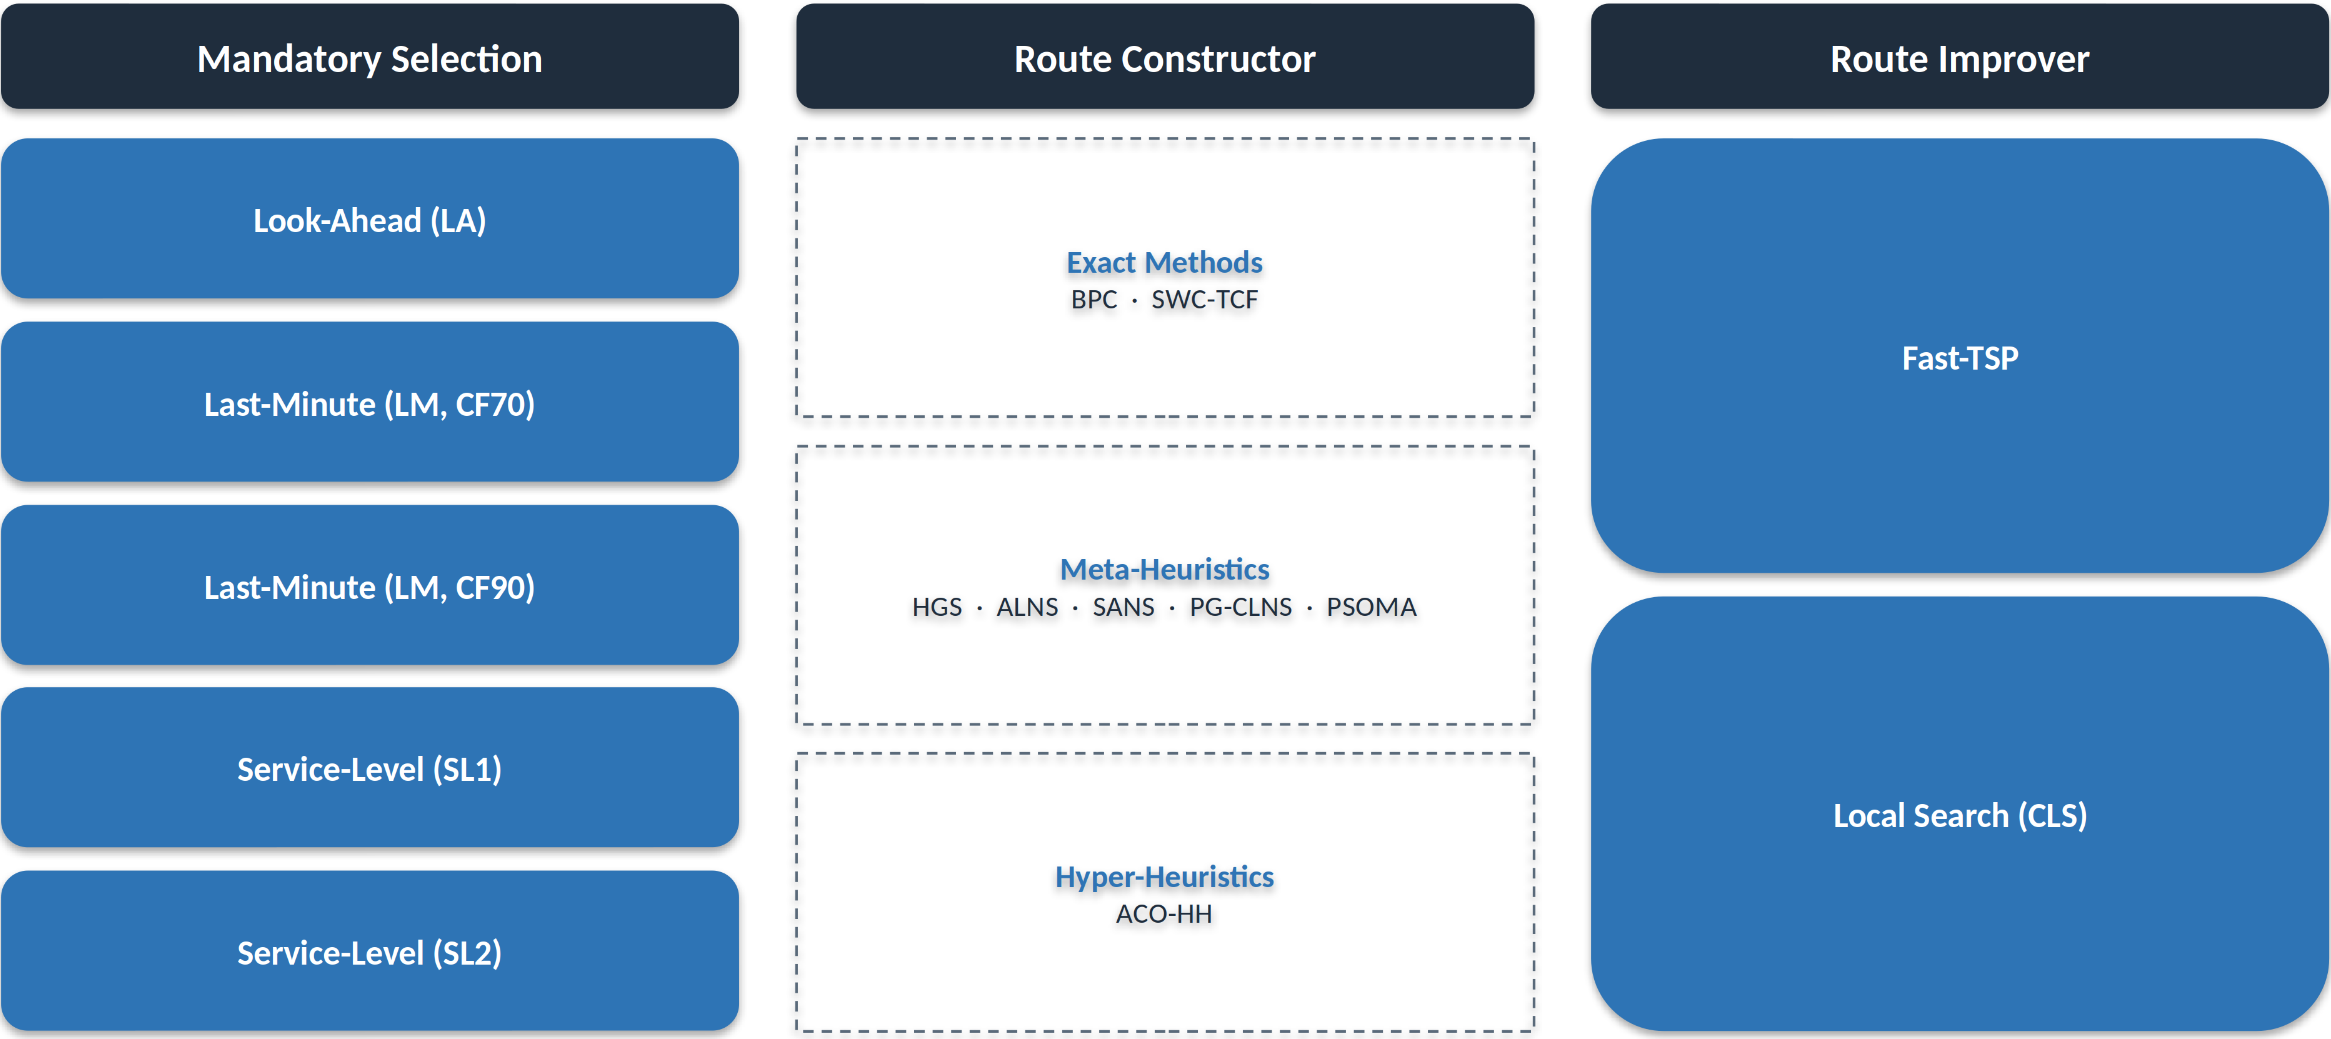
\includegraphics[width=1.0\linewidth]{Images/policy_configuration_space.png}
    \caption{Diagram of the routing policies considered for this work.}
    \label{fig:pol_config}
\end{figure}

\subsection{Mandatory Selection Strategies}

We considered three mandatory selection strategies. The simplest is the Last-Minute, where the mandatory bins are those whose predicted fill level at the end of the day is above a certain threshold. We tested with thresholds of 70\% (CF70) and 90\% (CF90). A second strategy is the Service Level one, which has the main goal of avoiding waste overflows, which has the number of days 

\subsection{Route Constructors}
\subsubsection{Exact Methods}
\paragraph{Smart Waste Collection - Two-Commodity Flow (SWC-TCF)}
The SWC-TCF was an algorithm introduced in \cite{RAMOS2018146}, which models the VRPP using a two-commodity flow formulation where the flow of at each bin is two times the amount of the bin's current waste fill.

\paragraph{Branch-Price-and-Cut (BPC)}
Write something about the BPC exact route constructors...

\subsubsection{Meta-Heuristics}
\paragraph{Adaptive Large Neighborhood Search (ALNS)}
The Adaptive Large Neighborhood Search (ALNS) extends the Large Neighborhood Search framework by dynamically selecting destroy and repair operators based on their past performance. At each iteration, a \textit{destroy} operator removes $q$ customers from the current solution, and a \textit{repair} operator reinserts them to form a new candidate solution.

For the VRPP, specific operators are designed to manage the selection of profitable nodes. Destroy operators may target nodes with low profit-to-cost ratios, while repair operators prioritize the insertion of high-profit nodes that incur minimal detour costs.

The selection of operator $i$ is governed by a roulette-wheel mechanism, where the probability $P(i)$ depends on its accumulated weight $w_i$. The weights are updated adaptively after each segment of $\varphi$ iterations:
\begin{equation}
    w_{i,t+1} = \lambda w_{i,t} + (1-\lambda) \frac{\pi_i}{\theta_i}
\end{equation}
where $\lambda \in [0, 1]$ is a decay factor, $\pi_i$ is the accumulated score of operator $i$ during the segment, and $\theta_i$ is the number of times it was used. Scores are awarded based on the quality of the new solution (e.g., finding a new global best).

\paragraph{Hybrid Genetic Search (HGS)}
The Hybrid Genetic Search (HGS) combines the evolutionary principles of a genetic algorithm with the fine-tuning capabilities of local search. The algorithm maintains a population of solutions, including feasible and infeasible individuals, to navigate the search space effectively. The core components include:
\begin{itemize}
    \item \textbf{Crossover:} An Ordered Crossover (OX) or similar operator generates offspring by inheriting routes from two parent solutions. In the context of VRPP, the crossover must ensure that the offspring respects the profit collection objectives.
    \item \textbf{Local Search (Education):} Each offspring undergoes an intensive local search procedure (e.g., 2-opt, Relocate, Swap) to reach a local optimum.
    \item \textbf{Population Management:} Diversity is strictly maintained by penalizing solutions that are too similar to existing ones, preventing premature convergence.
\end{itemize}
The fitness $F(S)$ of a solution $S$ is a weighted sum of its cost $C(S)$ and a diversity contribution $D(S)$:
\begin{equation}
    F(S) = C(S) + (1 - \frac{|P_{feas}|}{|P|}) \cdot D(S)
\end{equation}
where $|P_{feas}|$ is the number of feasible individuals in the population $P$.

\paragraph{Simulated Annealing Neighborhood Search (SANS)}
Write something about the SANS meta-heuristic route constructor...

\paragraph{Pheromone Guided - Cooperative Large Neighborhood Search (PG-CLNS)}
Write something about the PG-CLNS meta-heuristic route constructor...

\paragraph{Particle Swarm Optimization Memetic Algorithm (PSOMA)}
Write something about the PSOMA meta-heuristic route constructor...

\subsubsection{Hyper-Heuristics}
\paragraph{Hyper-Heuristic - Ant Colony Optimization (HH-ACO)}
While traditional Ant Colony Optimization (ACO) constructs solutions probabilistically based on pheromone trails, the Hyper-Heuristic ACO (HH-ACO) operates at a higher level of abstraction. Instead of directly building routes, the ants construct a sequence of low-level heuristics (LLH) to apply to the problem.

The problem state can be defined by the current solution quality or search stage. The ants probabilistically select heuristics based on a pheromone matrix $\tau_{sh}$ associated with state $s$ and heuristic $h$. The probability of choosing heuristic $h$ in state $s$ is given by:
\begin{equation}
    p_{sh} = \frac{[\tau_{sh}]^\alpha [\eta_{sh}]^\beta}{\sum_{k \in \mathcal{H}} [\tau_{sk}]^\alpha [\eta_{sk}]^\beta}
\end{equation}
where $\eta_{sh}$ is heuristic information indicating the potential efficacy of $h$, and $\alpha, \beta$ control the relative influence of pheromone and heuristic information. This allows the algorithm to learn essentially "which heuristic to apply when," adapting the search strategy specifically to the instance of the VRPP being solved.

\subsection{Route Improvers}
Route improvers are the last section of our modular routing policies, which receive an already constructed route (or set of routes) and fine-tunes the route node sequence to further increase routing efficiency. In this work, we made use of two different route improvement algorithms: Classical Local Search (CLS), which applies local search operators like 2-opt by increasing order of complexity, until no further improvement is found; and Fast-TSP, a Python library which underneath the hood implements a variation of Stochastic Local Search (SLC) for graph instances with more than 20 nodes.

\section{Experimental Evaluation}
We evaluate the models on a scenario where, given a statistical distribution, and the coordinates of a depot and multiple recycling bins, a simulator generates an amount of waste to fill each bin for ${d=\{31, 93, 365\}}$ days. Each day, the models are tasked with selecting which bins the recycling vehicle(s) are to collect waste from, a task which can be interpreted as a type of CO problem.

\subsection{Data}
During the evaluation process, we use the following statistical distributions and data sources (alternatives include \cite{brouwer2023comparison}):
\begin{itemize}
    \item Gamma distribution, and files with the coordinates and the waste accumulation rate of ${b_1=\{20, 50, 225\}}$ bins;
    \item Empirical distribution (WSmart+ Bin Analysis module), and two files with the coordinates of $b_2={317}$ bins and how much waste was generated each day for each bin (from 2021-01-12 to 2023-10-23), respectively.
\end{itemize}
We evaluate the models with ${V_{\Gamma}=20, 50, 100, 150, 225}$ bins on the Gamma distribution and ${V_{E}=20, 50, 100, 150, 225, 317}$ bins on the Empirical distribution. When $V_{\Gamma} \in V_1 \lor V_{E}=V_2$, we run a single simulation with bins available in the coordinates data file. Otherwise, we randomly sample $V_{\Gamma} = \{100, 150\}$ or $V_{E} = \{20, 50, 100, 150, 225\}$ bins for $N_s=100$ or $N_s=10$ samples, respectively.\\
Parameters for the Gamma distribution:
\begin{itemize}
    \item Gamma 1: alpha = [5, 5, 5, 5, 5, 10, 10, 10, 10, 10], beta =[5, 2]
        \subitem mean = [25, 10, 50, 20]
        \subitem variance = [125, 20, 250, 40]
    \item Gamma 2: alpha = [2, 2, 2, 2, 2, 6, 6, 6, 6, 6], beta = [6, 4]
        \subitem mean = [12, 8, 36, 24]
        \subitem variance = [72, 32, 216, 96]
    \item Gamma 3: alpha = [1, 1, 1, 1, 1, 3, 3, 3, 3, 3], beta = [8, 6]
        \subitem mean = [8, 6, 24, 18]
        \subitem variance = [64, 36, 192, 108]
\end{itemize}
The daily generated waste data from the WSmart+ Bin Analysis module is pre-processed to compute the waste accumulation rate of each bin.

\subsubsection{Map}
The map of the $V=317$ bins' coordinates can be seen in Figure \ref{fig:map}.
\begin{figure}
    \centering
    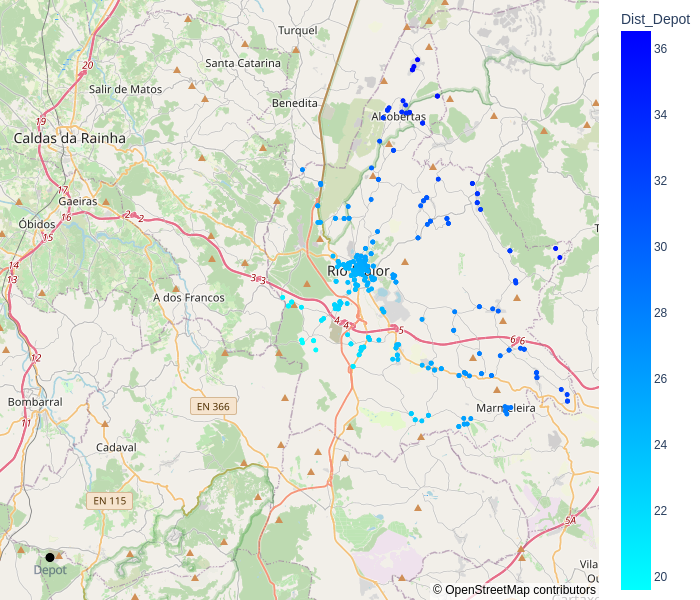
\includegraphics[width=0.75\linewidth]{Images/map317.png}
    \caption{Map of the depot and the 317 bins used in experiments.}
    \label{fig:map}
\end{figure}

\subsubsection{Baselines}
We will compare the proposed models with some state-of-the-art algorithms proposed recently, including: \textsc{look\_ahead\_policy} \cite{jorge2022hybrid}; \textsc{policy\_lastminute} \cite{lopes2023efficient}; \textsc{gurobi} \cite{de2024data}; and \textsc{policy\_regular}, where each location is visited regularly with an interval of 3 days, following a route computed by a TSP solver.

\subsection{Results}
\subsubsection{Gamma Distribution (31 days)}
Comparison of the algorithms and models' efficiency (kg/km) and the number of times a bin overflows with waste (overflows) for ${b_{\Gamma}=20, 50, 100, 150, 225}$ \ref{fig:log_gamma31}.
\begin{figure}
    \centering
    
\includegraphics[width=0.7\textwidth]{Images/Results/Gamma/31days/log_comp.png}
    \caption{Experimental results for Gamma distribution (with logarithmic scale on the Y axis and normalized by the number of days).}
    \label{fig:log_gamma31}
\end{figure}\\
Simulation runtime (time): \ref{fig:g31_logtime}\\
Number of bin waste collections (ncol): \ref{fig:g31_ncols}
\begin{figure}
    \centering
    
\includegraphics[width=0.49\linewidth]{Images/Results/Gamma/31days/log_time.png}
    
\includegraphics[width=0.49\linewidth]{Images/Results/Gamma/31days/ncol.png}
    \caption{(Left) Time (in seconds) it took to complete the simulation (with logarithmic scale on the Y axis and normalized by the number of days). (Right) Total number of bins collected during the simulation (normalized by the number of days).}
    \label{fig:g31_logtime}
    \label{fig:g31_ncols}
\end{figure}\\
In terms of truck capacity efficiency (kg/km) and the amount of waste overflows, the \textsc{attention model} seems to be the best option when it comes to smaller graphs, but \textsc{gurobi} eventually overtakes it as the best algorithms as we increase the number of bins in the simulation.\\
The \textsc{attention model} can output a solution to a problem instance in just a few seconds of inference time, making it the fastest algorithm by far. This is to be expected, as the model performs multiple parallel computations on the GPU, while the other algorithms are not parallelizable and must thus run on a single CPU thread. While significantly slower in comparison, both the \textsc{policy\_regular} and the \textsc{policy\_lastminute} can output a solution in a respectable time frame, taking around 1 to 3 minutes for graphs with $b \geq 100$. The \textsc{look\_ahead\_policy} and \textsc{gurobi} are - by a wide margin - the slowest of all algorithms, taking up to 3500x and 17000x more time than the attention model, respectively, to finish the simulation for 225 bins.\\
Overall, the attention model seems to offer the best runtime and performance in small graphs, while \textsc{gurobi} always offers a solid performance and is the superior algorithm for larger graphs with the trade-off of having a significantly higher runtime and computational cost. Also, \textsc{look\_ahead\_policy} seems to offer no significant performance benefits when compared to other algorithms and is the second most costly algorithm, making it a worse choice regardless of the metric.

\subsubsection{Gamma Distribution (365 days)}
Some results for 20 bins: \ref{fig:enter-label}\\
Some tours for 20 bins: \ref{fig:tours}
\begin{figure}
    \centering
    
\includegraphics[width=\linewidth]{Images/comp.png}
    \caption{For gamma dist 1 on 365 days.}
    \label{fig:enter-label}
\end{figure}
\begin{figure}
    \centering
    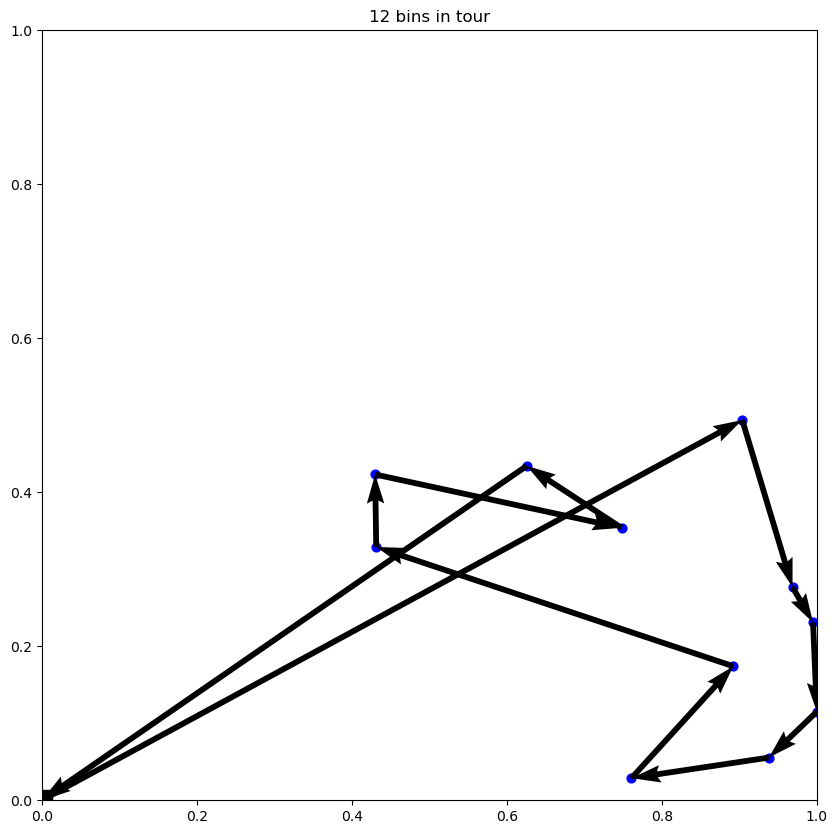
\includegraphics[width=0.49\textwidth]{Images/am_tour.png}
    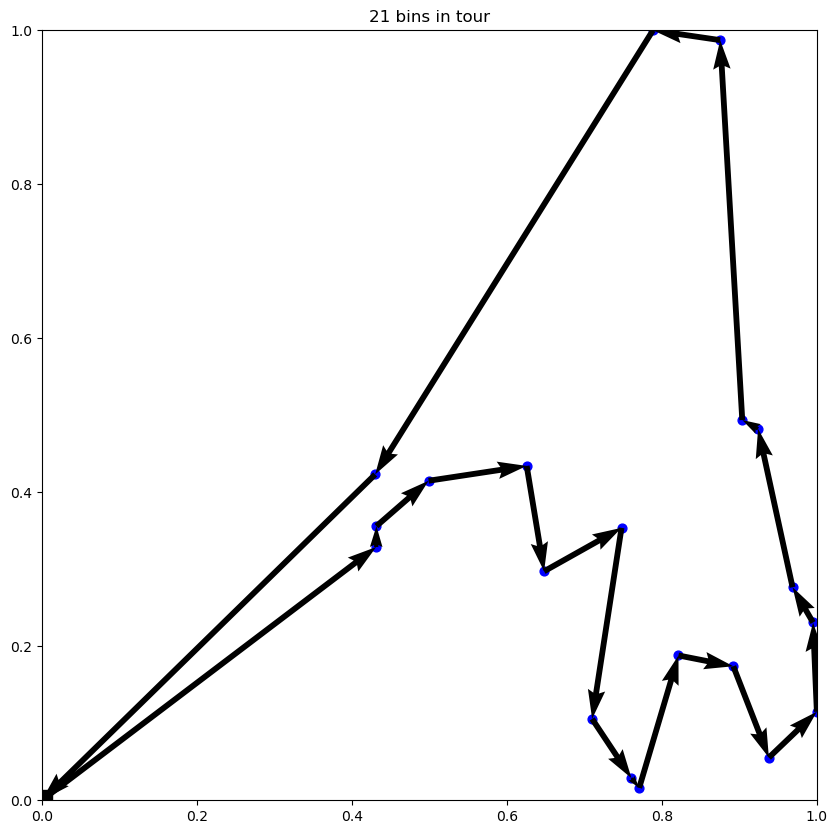
\includegraphics[width=0.49\textwidth]{Images/lookahead_tour.png}
    \caption{Example tours for Attention Model (left) and LookAhead Policy (right).}
    \label{fig:tours}
\end{figure}

\subsubsection{WSmart+ Bin Analysis (93 days)}
Comparison of the algorithms and models' efficiency (kg/km) and the number of times a bin overflows with waste (overflows) for ${b_{\Gamma}=20, 50, 100, 150, 225, 317}$ \ref{fig:log_emp93}.
\begin{figure}
    \centering
    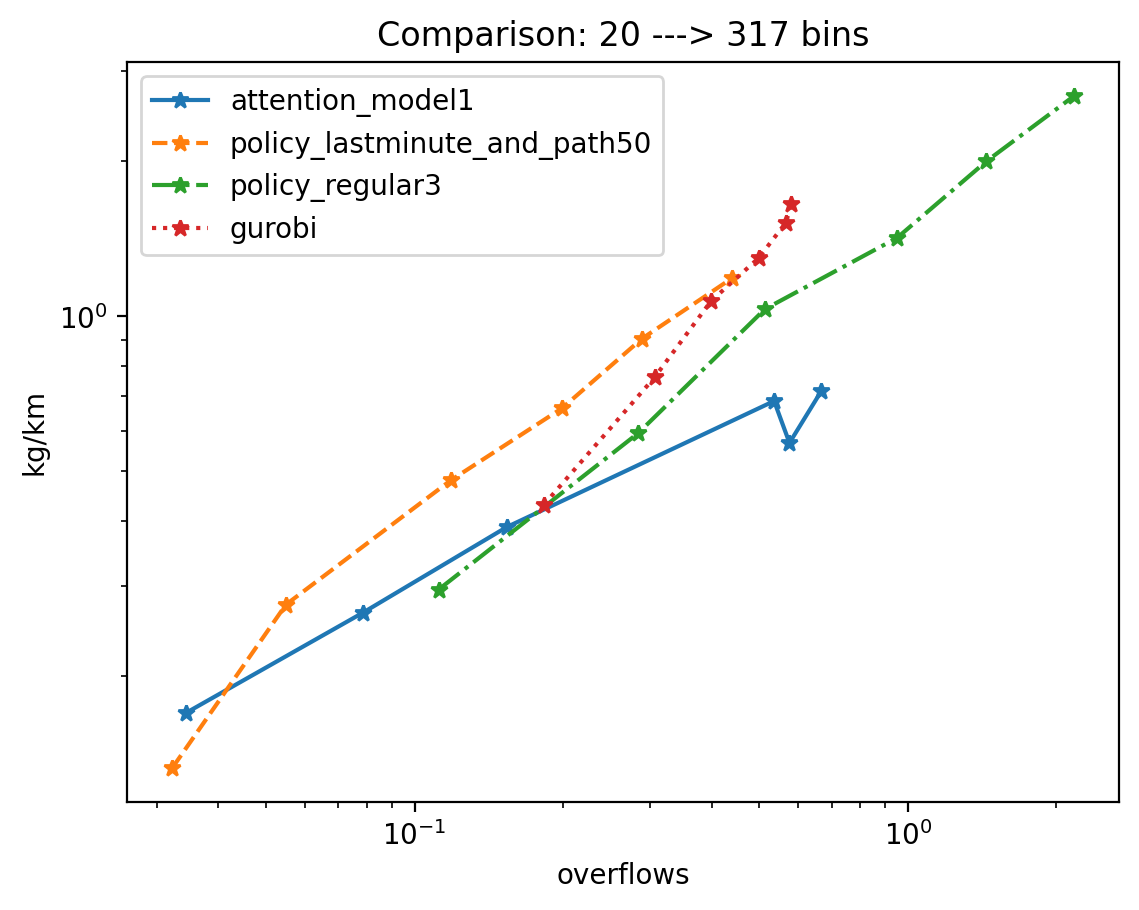
\includegraphics[width=0.49\textwidth]{Images/Results/Empirical/93days/log_comp.png}
    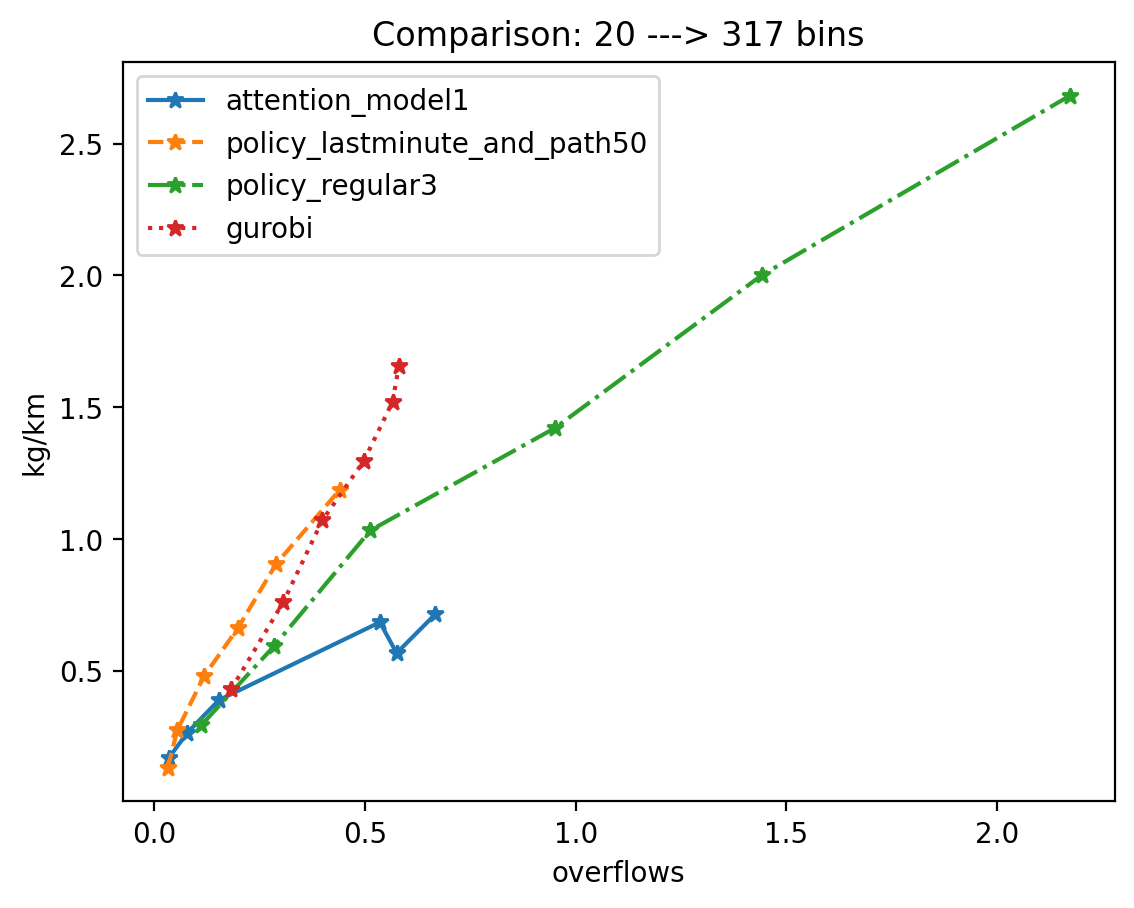
\includegraphics[width=0.49\textwidth]{Images/Results/Empirical/93days/comp.png}
    \caption{Experimental results for Gamma distribution (with logarithmic scale on both axes and normalized by the number of days).}
    \label{fig:log_emp93}
\end{figure}\\
Simulation runtime (time): \ref{fig:e93_logtime}\\
Number of bin waste collections (ncol): \ref{fig:e93_ncols}
\begin{figure}
    \centering
    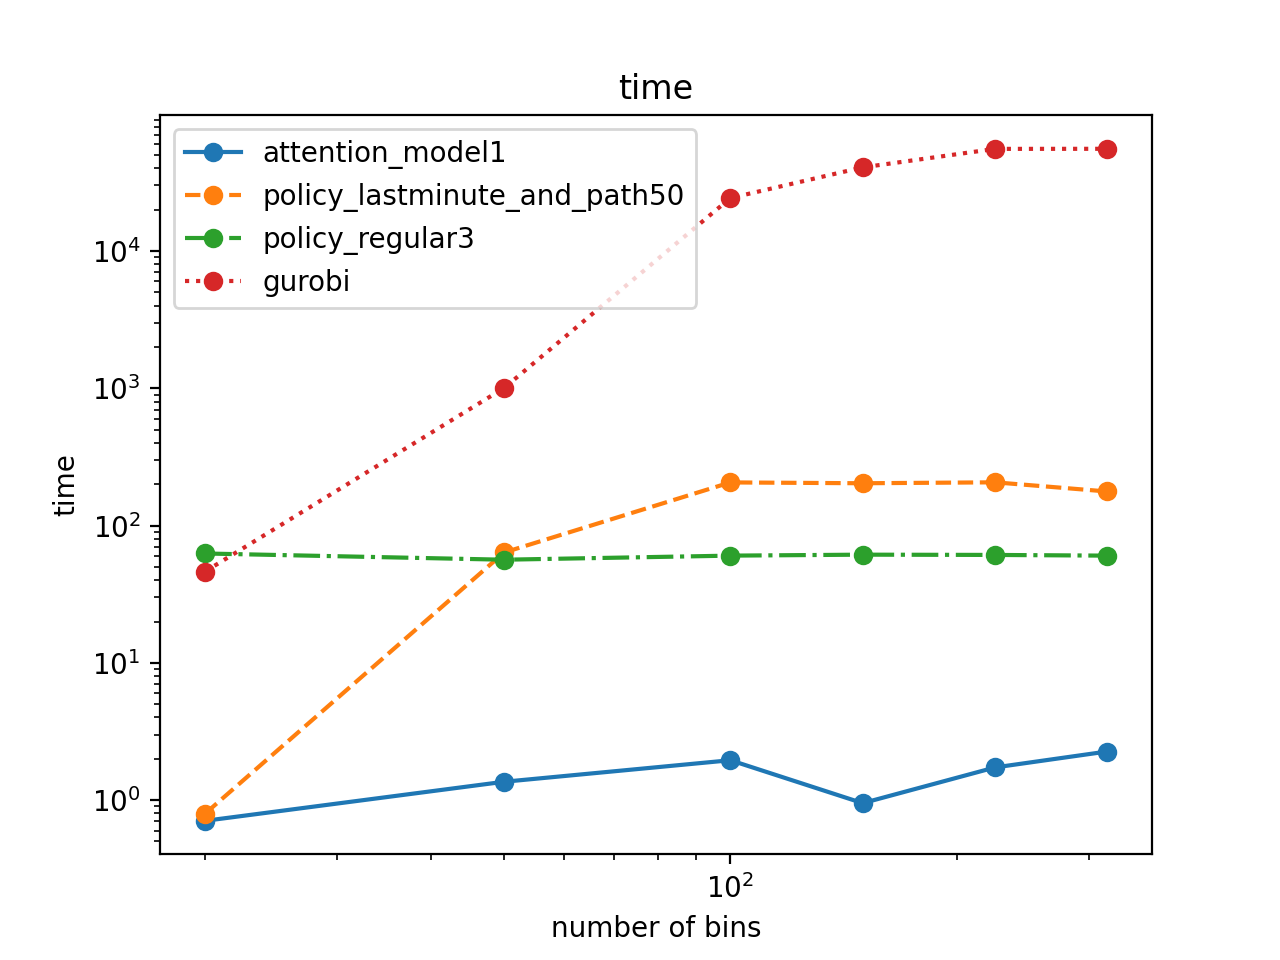
\includegraphics[width=0.49\linewidth]{Images/Results/Empirical/93days/log_time.png}
    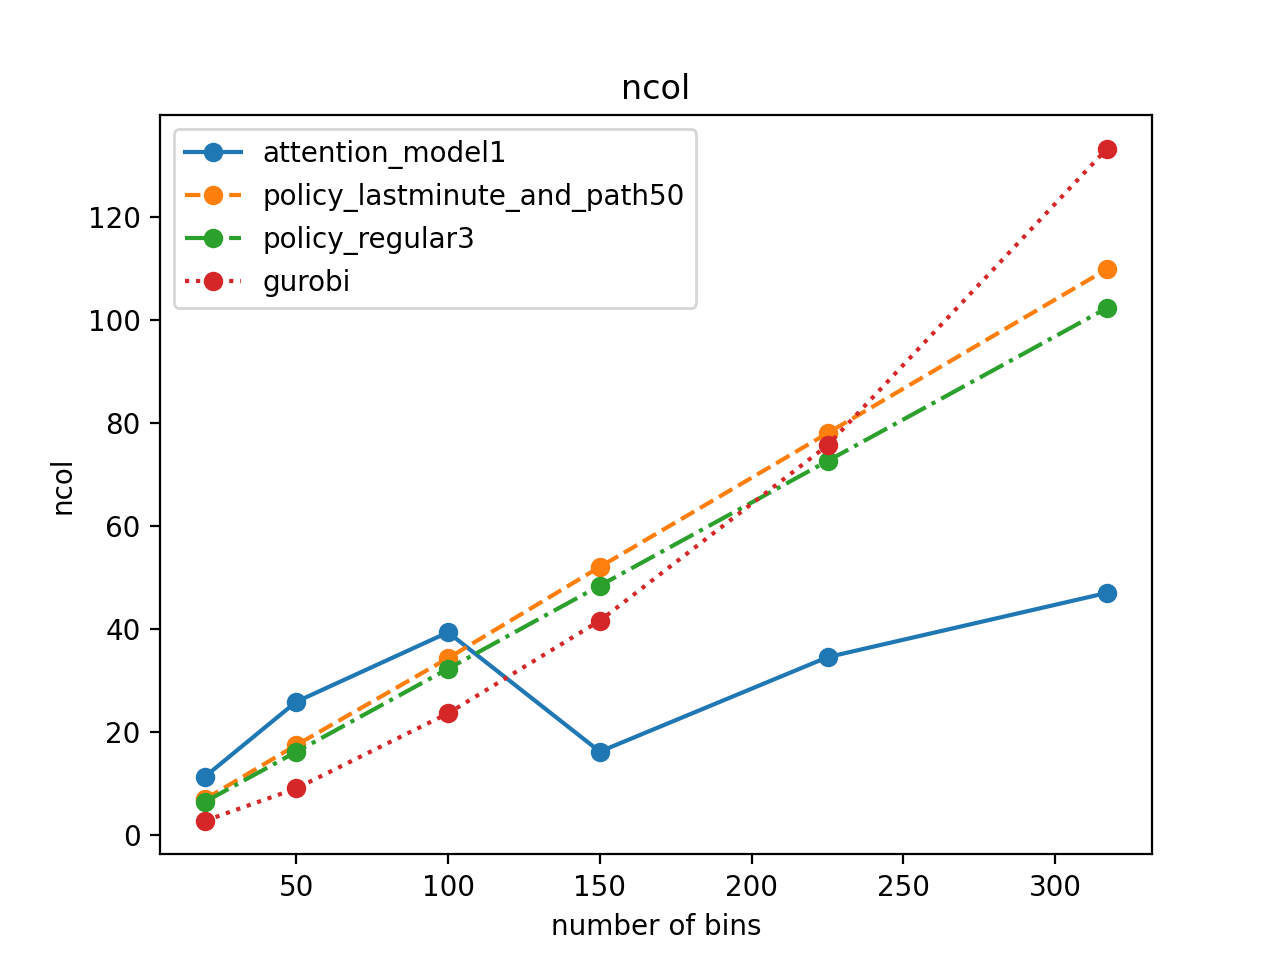
\includegraphics[width=0.49\linewidth]{Images/Results/Empirical/93days/ncol.png}
    \caption{(Left) Time (in seconds) it took to complete the simulation (with logarithmic scale on both axes and normalized by the number of days). (Right) Total number of bins collected during the simulation (normalized by the number of days).}
    \label{fig:e93_logtime}
    \label{fig:e93_ncols}
\end{figure}\\
Interestingly, the results seem to differ significantly from previous experiments when it comes to truck capacity efficiency (kg/km) and the amount of waste overflows. Compared to the results for the Gamma distribution, \textsc{gurobi} is no longer the most conservative algorithm with regards to the number of overflows and has an higher truck capacity efficiency. Also, the \textsc{policy\_lastminute} algorithm is extremely competitive in this scenario, achieving the best results in medium-sized graphs ($50 \leq b < 225)$.\\
The runtime results follow the same pattern as in the previous experiments, with the \textsc{attention model} being the fastest algorithm, followed by the \textsc{policy\_regular} and the \textsc{policy\_lastminute}, with the slowest of all being \textsc{gurobi}.

\section{Conclusion and Future Work}
Should write some text here after finishing up the Experimental Evaluation.

\begin{credits}
\subsubsection{\ackname} This study was funded by the WSmart Route+ project (grant number BI|2024/549), and carried out at INESC-ID.

\subsubsection{\discintname}
The authors have no competing interests to declare that are
relevant to the content of this article.
\end{credits}
%
% ---- Bibliography ----
%
% BibTeX users should specify bibliography style 'splncs04'.
% References will then be sorted and formatted in the correct style.
%
\bibliographystyle{splncs04}
\bibliography{mybibliography}

\end{document}
